In both of our extrapolation frameworks, we deliberately considered every available frequency to predict the ground-state energy, since we wanted to obtain a more general extrapolation. This "black-box" behaviour could lead to worse predictions, but does not require a hand-selection of a subset of the sequences for extrapolation. Also, this would require a metric on what sequences to choose. For ground-state energies, the convergence is monotonic and decreasing, such that we \textit{could} choose such a metric, where we choose the three sequences, for which the value at the highest $N_\mathrm{max}$ are the lowest among all sequences available. We want to demonstrate this frequency preselection idea by evaluating the \n{2}{H} nucleus using the same interaction as in the previous chapters with a flow parameter of \srg{0.08}. In \autoref{fig:eval_freqselection}, the results are shown. If we compare the results to the results of the unmodified training in \autoref{fig:eval_diff} for the \srg{0.08} interaction of \n{2}{H}, we can see that the frequency preselection significantly improves the absolute value, as well as the uncertainty of the prediction for the $N_\mathrm{max}$ values of $8$ and $10$.
\begin{figure}[H]
  \centering
  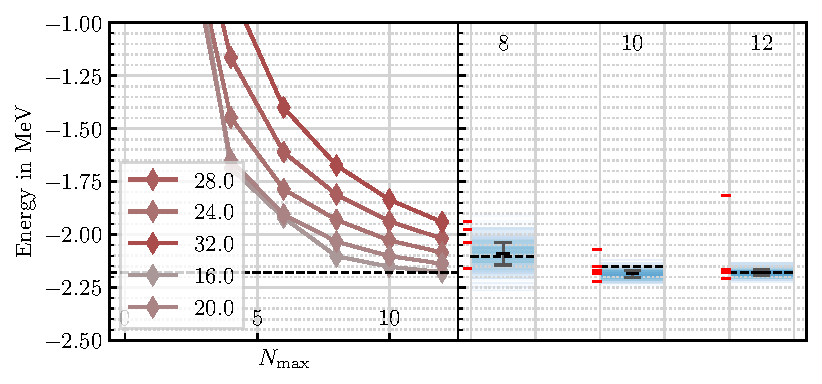
\includegraphics{media/outlook_selection.pdf}
  \caption{Evaluation of the \n{2}{H} nucleus in the difference based framework using only the three lowest frequencies. In this case, the frequencies are $\hbar\Omega = 16, 20, \SI{24}{\mega\electronvolt}$.}
  \label{fig:eval_freqselection}
\end{figure}
